\documentclass[runningheads]{llncs}

\usepackage{graphicx}
\usepackage{float}

\newcommand{\ignore}[1]{}

\floatstyle{ruled}
\floatname{algorithm}{Algorithm}
\newfloat{algorithm}{t}{}

\begin{document}

\title{Designing Oligonucleotide Microarrays (provisional title)}
%
% abbreviated title (for running head) also used for the TOC unless \toctitle is used
\titlerunning{Designing Oligonucleotide Microarrays}
%
\author{Sergio A. de Carvalho Jr.\inst{1,}\inst{2}\inst{,3} \and Sven Rahmann\inst{1,}\inst{3}}
%
% abbreviated author list (for running head)
\authorrunning{de Carvalho Jr. and Rahmann}
%
%%%% modified list of authors for the TOC (add the affiliations)
\tocauthor{Sergio A. de Carvalho Jr. (Universit\"{a}t Bielefeld),
Sven Rahmann (Universit\"{a}t Bielefeld)}
%
\institute{
International NRW Graduate School in Bioinformatics and Genome Research
\and
Graduiertenkolleg Bioinformatik, Bielefeld University, Germany \\
\email{Sergio.Carvalho@cebitec.uni-bielefeld.de}
\and
Algorithms and Statistics for Systems Biology group, Genome Informatics,
Technische Fakult\"at, Bielefeld University, D-33594 Bielefeld, Germany \\
\email{Sven.Rahmann@cebitec.uni-bielefeld.de}
}

% typeset the title of the contribution
\maketitle

% The abstract should summarize the contents of the paper
% using at least 70 and at most 150 words. It will be set in 9-point
% font size and be inset 1.0 cm from the right and left margins.
% There will be two blank lines before and after the Abstract.
\begin{abstract}
The production of commercial DNA microarrays is based on a
light-directed chemical synthesis driven by a set of masks or
micromirror arrays. Because of the natural properties of light and the
ever shrinking feature sizes, the arrangement of the probes on the
chip and the order in which their nucleotides are synthesized play an
important role on the quality of the final product. We propose a new
model called \emph{conflict index} for evaluating microarray layouts.
\end{abstract}

% ==============================================================================
\section{Introduction}
% ==============================================================================
\label{sec:intro}

An oligonucleotide microarray is a piece of glass or plastic on which
single-stranded fragments of DNA, called \emph{probes}, are affixed or
synthesized. Affymetrix GeneChip\raisebox{.6ex}{\scriptsize \textregistered}
arrays, for instance, can contain
more than one million spots (or \emph{features}) as small as 11 $\mu$m,
with each spot accommodating several million copies of a probe. Probes
are typically 25 nucleotides long and are synthesized on the chip, in parallel,
in a series of repetitive steps. Each step appends the same
nucleotide to probes of selected regions of the chip. Selection occurs
by exposure to light with the help of a photolithographic mask that
allows or obstructs the passage of light accordingly \cite{FODOR91}.

Formally, we have a set of probes $\mathcal{P} = \{p_{1}, p_{2}, ... p_{n}\}$
that are produced by a series of masks $\mathcal{M} = (m_{1}, m_{2}, ... m_{\mu})$,
where each mask $m_{k}$ induces the addition of a particular nucleotide
$t_{k} \in \{A, C, G, T\}$ to a subset of~$\mathcal{P}$. The \emph{nucleotide
deposition sequence} $\mathcal{S} = t_{1} t_{2} \ldots t_{\mu}$ corresponding
to the sequence of nucleotides added at each masking step is therefore a
supersequence of all $p_{i} \in \mathcal{P}$ \cite{RAHMANN03}.

In general, a probe can be \emph{embedded} within $\mathcal{S}$ in several
ways. An embedding of $p_{i}$ is a $\mu$-tuple
$\varepsilon_{i} = (e_{i,1}, e_{i,2}, ... e_{i,\mu})$ in which $e_{i,k} = 1$
if probe $p_{i}$ receives nucleotide $t_{k}$ (at step~$k$), or 0 otherwise
(Fig.\,\ref{fig:masking_process}). In particular, a \emph{left-most embedding}
is an embedding in which the bases are synthesized as soon as possible.

\begin{figure}
\centerline{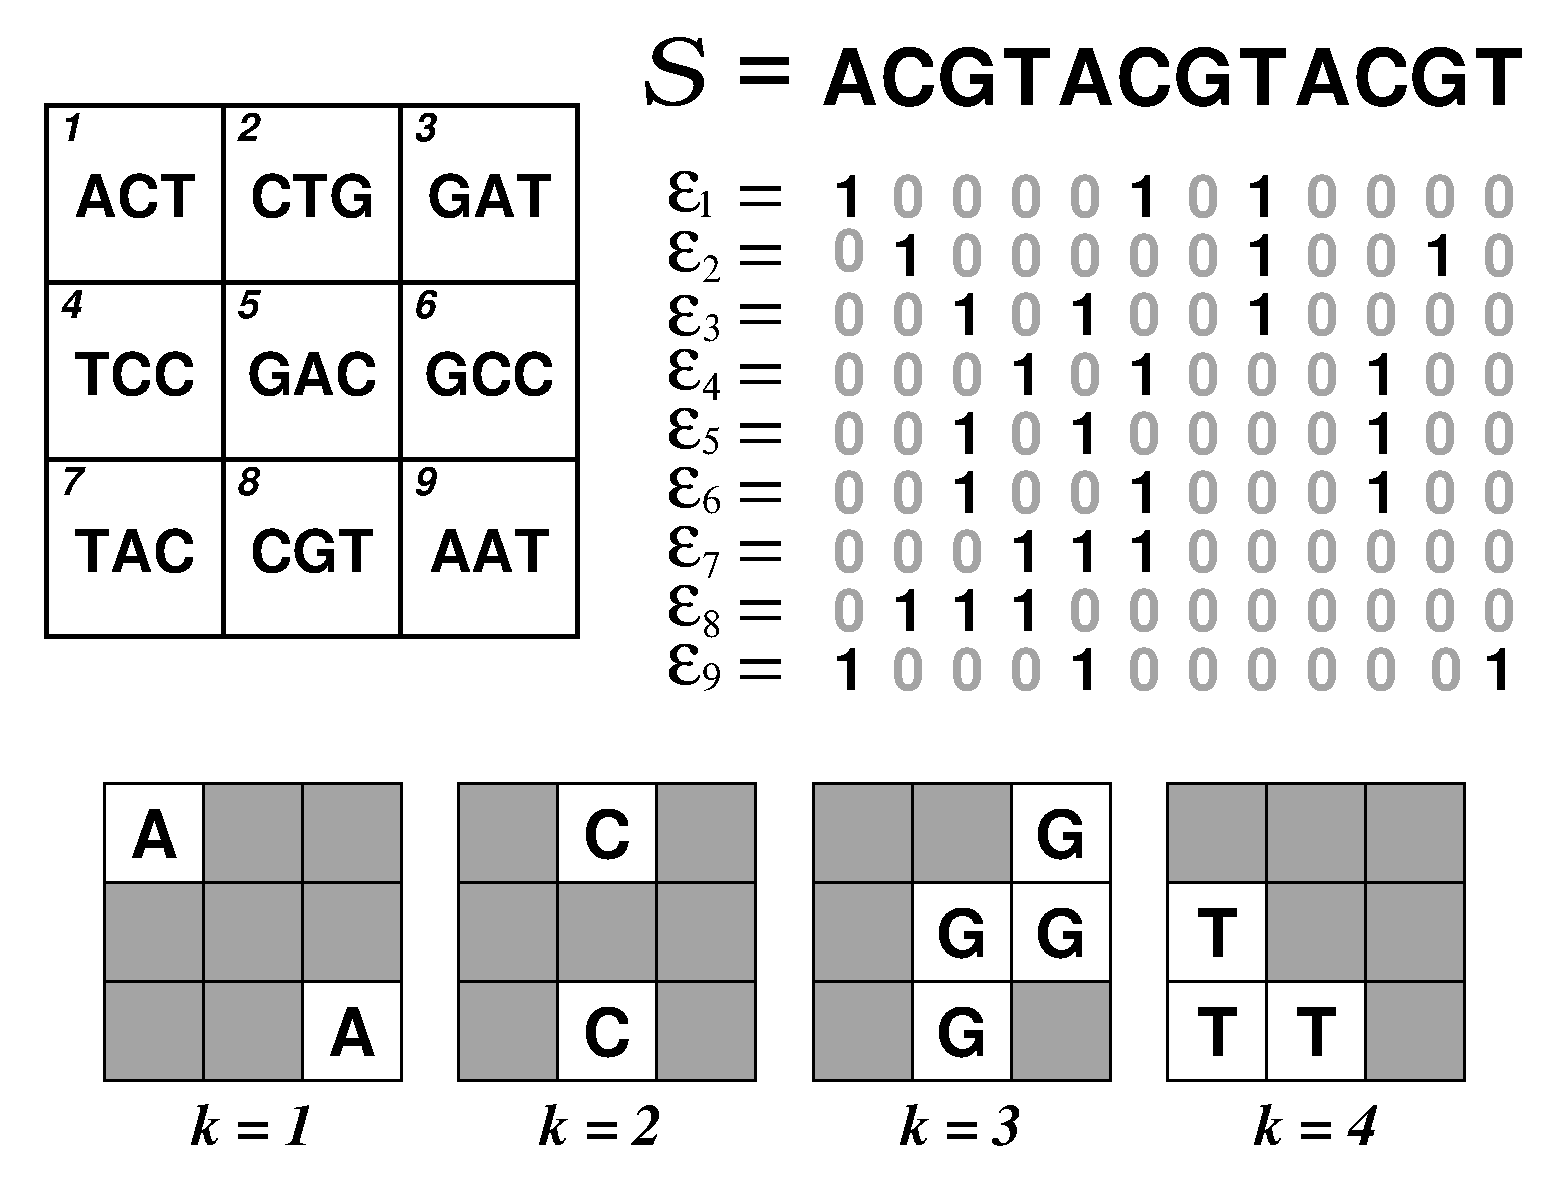
\includegraphics[width=230pt]{chip}}
\caption{Synthesis of a hypothetical 3\,x\,3 chip. On the top left, the chip
layout and its 3-base-long probe sequences. On the top right, the deposition
sequence and the probe embeddings. On the bottom, the first four resulting masks.}
\label{fig:masking_process}
\end{figure}

Deposition sequences are usually cyclical, that is $\mathcal{S}$, is a repeated
permutation of the alphabet. \ignore{This is mainly because such sequences maximize the
number of possible subsequences \cite{CHASE76}}. In this context, we can
distinguish between \emph{synchronous} and \emph{asynchronous} embeddings. In
the first case, each probe has one and only one nucleotide synthesized in every
cycle of the deposition sequence; hence, 100 masking steps are needed to
synchronously synthesize probes of length 25.
In the case of asynchronous
embeddings, probes can have any number of nucleotides synthesized in any given
cycle. This allows for shorter deposition sequences. All Affymetrix chips that
we know of can be asynchronously synthesized in 74 masking steps.

% removed footnote
\ignore{We
understand that Affymetrix uses the same truncated repetition of TGCA to
synthesize most (if not all) GeneChip arrays, which suggests that their probe
selection procedure is restricted to sequences that fit into this deposition
sequence.}

Because of diffraction of light or internal reflection, untargeted spots can
sometimes be accidentally activated in a certain masking step, producing
unpredicted probes that can compromise the results of an experiment. This problem
is more likely to occur near the borders between masked and unmasked
spots~\cite{FODOR91}. This observation has
given rise to the term \emph{border conflict}.

We are interested in finding an arrangement of the probes on the chip together
with their embeddings in such a way that the chances of unintended
illumination during mask exposure steps is minimized. This problem appears to
be hard because of the exponential number of possible arrangements,
although we are not aware of an NP-hardness proof.
In a separate work~\cite{CARVALHO06}, we presented a formulation based on
the quadratic assignment problem (QAP), a classical combinatorial optimization
problem that is known to be NP-hard and NP-hard to approximate. Our formulation
gives further indication that the problem is hard.

Optimal solutions are thus
unlikely to be found even for very small chips, and even if we consider the probes
as having a single pre-defined embedding.
If we consider all possible embeddings, the problem is even
harder. Affymetrix probes, for instance, can have up to several million different
embeddings. For this reason, the problem has been traditionally tackled in two
phases. First, an initial embedding of the probes is fixed and an arrangement of
these embeddings on the chip with minimum border conflicts is sought. This is
usually referred to as the \emph{placement}. Second, a \emph{post-placement}
optimization phase re-embeds the probes considering its location on the chip,
in such a way that the conflicts with the neighboring spots are further reduced.

\ignore{
We believe that better solutions can be found if, during the placement, we also
consider the various embeddings that a probe can have. In this paper we present
a new algorithm... % TODO continue...
}

In the next section, we review the Border Length Minimization Problem
\cite{HANNENHALLI02}, and define an extended model for evaluating microarray
layouts. In Sect.\,\ref{sec:previous_work}, we briefly review existing
placement strategies. % TODO finish this paragraph


% ==============================================================================
\section{Layout Evaluation}
% ==============================================================================
\label{sec:eval}

Hannenhalli~{\it et~al}.\ were the first to give a formal definition to the problem
of unintended illumination in the production of microarrays. They formulated the
\emph{Border Length Minimization Problem}\cite{HANNENHALLI02}, which aims at finding
an arrangement of the probes together with their embeddings in such a way that the number
of border conflicts during mask exposure steps is minimal.

The \emph{border length}~$\mathcal{B}_k$ of a mask~$m_{k}$ is simply
defined as the number of borders shared by masked and unmasked spots
at masking step~$k$. The total border length of a given arrangement is
the sum of border lengths over all masks. For example, the four masks
shown in Fig.\,\ref{fig:masking_process} have
$\mathcal{B}_1 = 4$, $\mathcal{B}_2 = 6$, $\mathcal{B}_3 = 6$ and $\mathcal{B}_4 = 4$.
The total border length of that arrangement is 50.

% ------------------------------------------------------------------------------
\subsection{Conflict Index}
\label{sec:conflict_index}

The border length of an individual mask measures the quality of that
mask. We are more interested in estimating the risk of synthesizing a faulty
probe at a given spot, that is, we need a per-spot measure
instead of a per-mask measure. Additionally, as noted by Kahng~{\it et~al}.~\cite{KAHNG03A},
the definition of border length does not take into account two
simple yet important practical considerations:
\begin{itemize}
\item[a)] stray light might activate not only adjacent neighbors but
  also probes that lie as far as three cells away from the targeted
  spot;
\item[b)] imperfections produced in the middle of a probe are more
  harmful than in its extremities.
\end{itemize}
This motivates the following definition of the \emph{conflict
  index}~$\mathcal{C}(s)$ of a spot~$s$ whose probe of
length~$\ell_{s}$ is synthesized in $\mu$~masking steps. First, we
define a distance-dependent weighting function, $\delta(s,s',k)$, that
accounts for observation a) above:
%%
\begin{equation}
\label{eq:dist_weight}
\delta(s,s',k) :=
        \left\{
                \begin{array}{ll}
                        (d(s,s'))^{-2} & \mbox{if $s'$ is unmasked at step $k$}, \\
                        0 & \mbox{otherwise}, \\
                \end{array}
        \right.
\end{equation}
%%
where $d(s,s')$ is the Euclidean distance between spots~$s$ and~$s'$.
This form of weighting function is the same as suggested in
\cite{KAHNG03A}.  Note that $\delta$ is a ``closeness'' measure
between $s$ and $s'$ only if $s'$ is
not masked (and thus creates the potential of illumination at $s$). To
restrict the number of neighbors that need to be considered, we
restrict the support of $\delta(s,s',\cdot)$ to those $s'\neq s$ that
are in a $7\times 7$ grid centered around $s$ (see
Fig.\,\ref{fig:conflictindex}~top).


We also define position-dependent weights to account for observation b):
%%
\begin{equation}\label{eq:pos_mult}
\omega(s,k) :=
\left\{
  \begin{array}{ll}
    c \cdot \exp{\left(\theta \cdot \lambda(s,k)\right)} & \mbox{if $s$ is masked at step $k$}, \\
    0 & \mbox{otherwise}, \\
  \end{array}
\right.
\end{equation}
%%
where $c>0$ and $\theta>0$ are constants, and
%%
\begin{equation}\label{eq:base_pos}
  \lambda(s,k) := 1 + \min(b_{s,k},\ell_{s} - b_{s,k})
\end{equation}
%%
is the distance of the nucleotide synthesized in step $k$ (if any)
from the start or end of the probe: $b_{s,k}$ denotes the number of
nucleotides synthesized at spot~$s$ up to and including step~$k$, and
$\ell_s$ is the probe length (see Fig.\,\ref{fig:conflictindex}
bottom). We set the constants $c$ and $\theta$ as follows:
\[ \theta = \frac{5}{\ell_s}; \qquad c = \frac{1}{\exp{\theta}}. \]
It is generally agreed that the chances of a successful hybridization
between probe and target are higher if a mismatched base occurs at the
extremities of the formed duplex instead of at its center. The precise
effects of this position, however, is not yet fully understood and has
been an active topic of research \cite{BINDER05}. The motivation
behind an exponentially increasing weighting function is that the
probability of a successful stable hybridization of a probe with its
target should increase exponentially with the absolute value of its
Gibbs free energy, which increases linearly with the length of the
longest perfect match between probe and target. The parameter $\theta$
controls how steeply the exponential weighting function rises towards
the middle of the probe.

We now define the conflict index of a spot $s$ as
\begin{equation}
\label{eq:conf_idx}
\mathcal{C}(s) := \sum_{k=1}^{\mu} \left( \omega(s,k) \sum_{s'} \delta(s,s',k) \right),
\end{equation}
%%
where $s'$ ranges over all spots that are at most three cells away
from $s$.  $\mathcal{C}(s)$ can be interpreted as the fraction of
faulty probes (because of unwanted illumination) produced at spot $s$.

\begin{figure}
\centerline{
%%
\begin{picture}(160,105)
\put(0,25){\makebox(160,80){
\begin{minipage}{160pt}
\centerline{\footnotesize{
\begin{tabular}{c|c|c|c|c|c|c|c|} \cline{2-8}
& \ 0.06 & \ 0.08 & \ 0.10 & \ 0.11 & \ 0.10 & \ 0.08 & \ 0.06 \\ \cline{2-8}
& \ 0.08 & \ 0.13 & \ 0.20 & \ 0.25 & \ 0.20 & \ 0.13 & \ 0.08 \\ \cline{2-8}
& \ 0.10 & \ 0.20 & \ 0.50 & \ 1.00 & \ 0.50 & \ 0.20 & \ 0.10 \\ \cline{2-8}
& \ 0.11 & \ 0.25 & \ 1.00 & \  s   & \ 1.00 & \ 0.25 & \ 0.11 \\ \cline{2-8}
& \ 0.10 & \ 0.20 & \ 0.50 & \ 1.00 & \ 0.50 & \ 0.20 & \ 0.10 \\ \cline{2-8}
& \ 0.08 & \ 0.13 & \ 0.20 & \ 0.25 & \ 0.20 & \ 0.13 & \ 0.08 \\ \cline{2-8}
& \ 0.06 & \ 0.08 & \ 0.10 & \ 0.11 & \ 0.10 & \ 0.08 & \ 0.06 \\ \cline{2-8}
\end{tabular}}}
\end{minipage}}}
\end{picture}
%%
\begin{picture}(190,105)
\footnotesize{
\put(0,0){\makebox(190,105){
  %GNUPLOT: LaTeX picture with Postscript
\begin{picture}(0,0)%
\includegraphics{position_weights}%
\end{picture}%
\begingroup
\setlength{\unitlength}{0.0200bp}%
\begin{picture}(9900,5940)(0,0)%
\put(1250,1500){\makebox(0,0)[r]{\strut{} 0}}%
\put(1250,2157){\makebox(0,0)[r]{\strut{} 2}}%
\put(1250,2813){\makebox(0,0)[r]{\strut{} 4}}%
\put(1250,3470){\makebox(0,0)[r]{\strut{} 6}}%
\put(1250,4127){\makebox(0,0)[r]{\strut{} 8}}%
\put(1250,4783){\makebox(0,0)[r]{\strut{} 10}}%
\put(1250,5440){\makebox(0,0)[r]{\strut{} 12}}%
\put(1647,1000){\makebox(0,0){\strut{} 0}}%
\put(3118,1000){\makebox(0,0){\strut{} 5}}%
\put(4589,1000){\makebox(0,0){\strut{} 10}}%
\put(6061,1000){\makebox(0,0){\strut{} 15}}%
\put(7532,1000){\makebox(0,0){\strut{} 20}}%
\put(9003,1000){\makebox(0,0){\strut{} 25}}%
%\put(5325,250){\makebox(0,0){\strut{}$b_{s,k}$}}%
\end{picture}%
\endgroup
\endinput

%%% Local Variables: 
%%% mode: latex
%%% TeX-master: t
%%% End: 

}}}
\end{picture}
%%
}
%\vspace*{-3ex}
\caption{Ranges of values for both $\delta$ and $\omega$ on a typical Affymetrix
chip where probes of length~$\ell = 25$ are synthesized in $\mu = 74$ masking
steps. Left: approximate values of the distance-dependent weighting function
$\delta(s,s',k)$ for a spot~$s$
(shown in the center) and close neighbors $s'$, assuming that $s'$ is unmasked
at step $k$. Right: position-dependent weights $\omega(s,k)$ at each value of
$b_{s,k}$, assuming that spot $s$ is masked at step $k$.}
\label{fig:conflictindex}
\end{figure}

\ignore{
\footnotesize{
\begin{tabular}{c|c|c|c|c|c|c|c|} \cline{2-8}
& \ 0.06 & \ 0.08 & \ 0.10 & \ 0.11 & \ 0.10 & \ 0.08 & \ 0.06 \\ \cline{2-8}
& \ 0.08 & \ 0.13 & \ 0.20 & \ 0.25 & \ 0.20 & \ 0.13 & \ 0.08 \\ \cline{2-8}
& \ 0.10 & \ 0.20 & \ 0.50 & \ 1.00 & \ 0.50 & \ 0.20 & \ 0.10 \\ \cline{2-8}
& \ 0.11 & \ 0.25 & \ 1.00 & \  s   & \ 1.00 & \ 0.25 & \ 0.11 \\ \cline{2-8}
& \ 0.10 & \ 0.20 & \ 0.50 & \ 1.00 & \ 0.50 & \ 0.20 & \ 0.10 \\ \cline{2-8}
& \ 0.08 & \ 0.13 & \ 0.20 & \ 0.25 & \ 0.20 & \ 0.13 & \ 0.08 \\ \cline{2-8}
& \ 0.06 & \ 0.08 & \ 0.10 & \ 0.11 & \ 0.10 & \ 0.08 & \ 0.06 \\ \cline{2-8}
\end{tabular}
}
}

Finally, we note the following relation between conflict indices and border
lengths. Define $\delta(s,s',k):=1$ if $s'$ is a direct neighbor of $s$ and is
unmasked in step $k$, and $:=0$ otherwise.  Also define $\omega(s,k):=1$ if
$s$ is masked in step $k$, and $:=0$ otherwise. Then $\sum_s\, \mathcal{C}(s)
= 2 \sum_{k=1}^\mu\, \mathcal{B}_k$, as each border conflict is counted twice,
once for $s$ and once for $s'$.

This shows that total border length and total conflict are correlated. A good
layout is one with low border length as well as low average conflict index,
although it is clearly possible to observe a reduction of the conflict index
at the expense of an increase in border length, and vice-versa.


% ==============================================================================
\section{Previous Work}
% ==============================================================================
\label{sec:previous_work}

\ignore{The first to formally address the border length problem were \cite{FELDMAN93}.
They showed how an optimal placement can be constructed based on a two-dimensional
Gray code. However, their work is restricted to \emph{uniform arrays} (arrays
containing all possible probes of a given length) and synchronous embeddings.}

Hannenhalli~{\it et~al}.\ \cite{HANNENHALLI02} were the first to consider the border
length problem on large
oligonucleotide arrays of arbitrary probes. They reported that the first Affymetrix
chips were designed using a heuristic for the traveling salesman problem (TSP). The
idea consists of building a weighted graph with nodes representing probes, and edges
containing the Hamming distance between the probe sequences. A TSP tour is approximated,
resulting in consecutive probes in the tour being likely to be similar. The TSP
tour is then \emph{threaded} on the array in a row-by-row fashion.
Hannenhalli~{\it et~al}.\ suggested a different threading of the TSP tour on the chip,
called \emph{1-threading}, to achieve up to 20\% reduction in border length.

% old version of paragraph about Epitaxial alg.
\ignore{
Kahng~{\it et~al}.~\cite{KAHNG02} propose the \emph{Epitaxial} placement algorithm that
places a random probe in the center of the array and continues to
insert probes in spots adjacent to already filled spots, employing a
greedy heuristic to select the next spot to be filled and the probe
that is assigned to it. Priority is given to spots whose
neighbors are already filled, in which case the algorithm places the
probe with minimum sum of Hamming distances to its neighbors. If no
such a spot exists, the algorithm examines all non-filled spots~$s_i$
with $n_i \geq 1$ filled neighbors and finds a non-assigned probe
$p_j$ with minimum sum of Hamming distances to the neighboring probes
$H_{ij}$. For each possible assignment of $p_j$ to $s_i$, it computes
a cost $c(s_i,p_j) := k_{n_i} H_{ij} / n$, where $k_{n_i}$ are scaling
coefficients ($k_1 = 1$, $k_2 = 0.8$, and $k_3 = 0.6$), and makes the
assignment with minimum cost. With this algorithm, they claimed to
achieve up to 10\% reduction in border conflicts over the TSP-based
approach of Hannenhalli~{\it et~al}.\ \cite{HANNENHALLI02}.
}

Kahng~{\it et~al}.~\cite{KAHNG02} propose the \emph{Epitaxial} placement algorithm that
places a random probe in the center of the array and continues to
insert probes in spots adjacent to already filled spots. Priority is given
to spots with the largests numbers of filled neighbors. At each iteraction,
it examines all non-filled spots~$s_i$ and finds a non-assigned probe
$p_j$ with minimum sum of Hamming distances to the neighboring probes
$H_{ij}$, employing a greedy heuristic to select the next spot to be filled.
With this algorithm, they claimed to
achieve up to 10\% reduction in border conflicts over the TSP+1-threading
approach of Hannenhalli~{\it et~al}.\ \cite{HANNENHALLI02}.

\ignore{
The major problem with the Epitaxial and the TSP-based algorithm is that they
have at least quadratic time complexity and thus are not scalable for the
latest million-probe microarrays. According to their experiments, the TSP
approach needed around 32 minutes to produce the layout of a 200\,x\,200
chip, whereas the Epitaxial algorithm needed 74 minutes on average. For a
500\,x\,500 chip, the TSP took over 30 hours to complete, whereas the
Epitaxial algorithm did not complete ``due to prohibitively large running
time or memory requirements'' \cite{KAHNG02}.
}

\ignore{
This observation has led to the development of two new algorithms by
\cite{KAHNG03A}. The first one, called Sliding-window Matching (SWM), is not
exactly a placement algorithm as it iteratively improves an initial placement
that can be constructed by, for instance, TSP and 1-threading. Improvements
are achieved by selecting an independent set of spots inside the window and
optimally replacing their probes using a minimum-weight perfect matching
algorithm. The term independent refers to probes that can be replaced without
affecting the border length of the other selected probes.
}

Both the Epitaxial algorithm and the TSP approach do not scale well to large
chips.  For this reason, Kahng~{\it et~al}.~\cite{KAHNG03A} propose a simpler variant
of the Epitaxial algorithm, called \emph{Row-epitaxial}, with two main
differences: spots are filled in a pre-defined order, namely
from top to bottom, left to right, and only probes of a limited list of candidates are
considered when filling each spot. Their experiments showed
that the Row-epitaxial is the best large-scale placement algorithm,
achieving up to 9\% reduction in border length over the TSP+1-threading.

\ignore{
The ever growing number of probes on the latest microarrays and the properties of
the placement problem naturally suggest the use of partitioning strategies to reduce
the running time of the algorithms.
}

\paragraph{Partitioning Algorithms.}
The placement problem can be trivially partitioned by
dividing the set of probes into smaller sub-sets, and assigning these sub-sets to
sub-regions of the chip. Each sub-region can then be treated as an independent chip
or recursively partitioned. These smaller sub-problems, when solved, immediately
constitute a final solution. In this way, algorithms with non-linear time or space
complexities can be used to compute the layout of larger chips that otherwise would not
be feasible. A partitioning is clearly a compromise in solution quality, but
for a large number of probes it can be minor.

The only known partitioning algorithm is the Centroid-based
Quadrisection~\cite{KAHNG03B}. It starts by randomly selecting a probe
$c_1 \in \mathcal{P}$. Then, it selects another probe $c_2$ maximizing
$h(c_1,c_2)$, the Hamming distance between their embeddings. Similarly, it selects
$c_3$ and $c_4$ maximizing the sum of Hamming distance between these four probes,
that are called centroids. All other probes
$p_i \in \mathcal{P}$ are then compared to the centroids and assigned to the sub-set
$\mathcal{P}_j$ associated with $c_j$ with minimum $h(p_i,c_j)$. The chip is divided
into four quadrants, each being assigned to a sub-set $\mathcal{P}_j$ .
The procedure is repeated
recursively on each quadrant until a given recursion depth is reached. In the end,
the Row-epitaxial algorithm is used to produce the placement of the probes in each
final sub-region.

\paragraph{Post-placement Optimization.}
Once the placement is done, further reduction of conflicts can be
achieved by re-embedding the probes without changing their locations.
Kahng~{\it et~al}.~\cite{KAHNG02} presented an efficient dynamic programming
algorithm, that we call Optimum Single Probe Embedding (OSPE), for computing an
optimum embedding of a probe on a spot $s$ in regards to the probes of
neighboring spots, whose embeddings are considered fixed.
Originally, it was developed for border length minimization, but
in Sect.\,\ref{sec:ospe}, we show how it can also be used for minimizing the
sum of conflict indices in the region around $s$.

The OSPE algorithm is the basic operation of several post-placement optimization
algorithms proposed by Kahng~{\it et~al}.: Batched Greedy~\cite{KAHNG02},
Chessboard~\cite{KAHNG02} and Sequential~\cite{KAHNG03B}. Their main difference lies in
the order in which the re-embeddings take place.

\ignore{
The first algorithm is a simple greedy approach that computes, for each spot of the chip,
the maximum reduction of conflicts that could be achieved by re-embedding its probe with
the OSPE algorithm. It then greedily selects the spot with higher gain and re-embeds
its probe optimally in regards to its neighbors, updating the gains of affected
spots. A faster version, called Batched Greedy, sacrifices its greedy nature by postponing
the update of gains and re-embedding all probes that have not been affected by the
re-embeddings performed in the current iteration.

The Chessboard optimization is based on the fact that a chip can be bi-colored
just like a chessboard, in such a way that the embeddings of probes located on
white spots, with respect to border length, are independent of those placed on black spots,
and vice-versa. The Chessboard uses this coloring to alternate the optimal re-embedding
of probes located on black and white spots.
}

The Sequential algorithm is a strikingly simple yet the most effective post-placement
optimization. It just proceeds spot by spot, from top to bottom, left to right,
re-embedding all probes with the OSPE algorithm. Surprisingly, it achieves the greatest
reduction of border conflicts with a running time compared to the Batched Greedy,
the faster among the three.

The OSPE algorithm can never increase the amount of conflicts in a region.
All optimization algorithms can thus be executed several times until
a local optimal solution is found, or until the improvements drop below a given threshold.

% ==============================================================================
\section{Optimum Single Probe Embedding}
% ==============================================================================
\label{sec:ospe}

The Optimum Single Probe Embedding~\cite{KAHNG02} is a dynamic programming
algorithm that computes the optimum embedding of a probe $p$ on a spot $s$
in regards to its neighboring probes whose embeddings are fixed. We first present
a general formulation for conflict index minimization; later we show the
formulation for border length minimization as a special case.

The OSPE can be seen as a special case of a global alignment between the
sequence $p$ of length $\ell$ and the deposition sequence $\mathcal{S}$ of length
$\mu$. We use an $(\ell + 1) \times (\mu + 1)$ array $D$ where the entry $D[i,j]$
contains the minimum cost of an embedding of $p[1..i]$ into $\mathcal{S}[1..j]$.
The cost is the sum of conflicts induced by the embedding of $p$ on its neighbors
plus the conflicts suffered by $p$ because of the embeddings of its neighbors.

At every step of the deposition sequence, the spot $s$ can be either masked or
unmasked. Thus, entry $D[i,j]$ is computed as the minimum between the costs
resulting from each possible action:
%%
\begin{equation}
D[i,j] = \min (D[i-1,j] + M_{ij}, D[i-1,j-1] + U_{j}),
\end{equation}
%%
where $M_{ij}$ is the cost of masking spot $s$ at step $j$ given that base $i$ of
probe $p$ has already been synthesized, and $U_{j}$ is the cost of unmasking spot
$s$ at step $j$.

If the spot $s$ is masked at a step $j$, any neighbor that is unmasked generates
a conflict on $p$ because it creates the potential of illumination at $s$. The
cost of such action is then set as follows:
%%
\begin{equation}
M_{ij} := c \cdot \exp{\left(\theta \cdot \lambda(s,k)\right)}
\end{equation}
%%
where $c$ and $\theta$ are constants, and $\lambda(s,k)$ is as defined
in~(\ref{eq:base_pos}).

Similarly, if the spot $s$ is unmasked at a step $j$, it may generate a conflict
on any neighbor $s'$ that is masked, and the cost of this action is set as follows:
%%
\begin{equation}
U_{j} := \sum_{s'} \omega(s',j) \cdot (d(s',s))^{-2},
\end{equation}
%%
where $d(s',s)$ is the Euclidean distance between spots~$s'$ and~$s$, and
$\omega(s',j)$ is as defined in~(\ref{eq:pos_mult}).

\paragraph{Border length minimization.} To do.

\paragraph{Remarks.}
The time complexity of the OSPE algorithm is $O(\ell_p \cdot |\mathcal{S}|)$,
where $\ell_p$ is the length of probe $p$ and $|\mathcal{S}|$ is the length of
the deposition sequence~\cite{KAHNG02}.

The three algorithms mentioned in Sect.\,\ref{sec:previous_work} were developed with
the aim of reducing border conflicts. The Batched Greedy and the Sequential algorithms,
however, can also be used to reduce the sum of conflict indices by using the OSPE as
decribed here.

% ==============================================================================
\section{Pivot Partitioning}
% ==============================================================================
\label{sec:pivotpart}

Traditionally, the microarray design problem has been tackled in two phases. First,
an initial embedding of the probes is fixed and an arrangement of these sequences
on the chip is produced by a placement algorithm. Then, a post-placement optimization
phase re-embeds the probes using the OSPE algorithm to achive further reduction in
conflicts. We believe that better layouts can be produced if the placement phase
also considers
the various embeddings that a probe can have. In this section we propose a new
partitioning algorithm called Pivot Partitioning (PP).

Our algorithm
has some similarities with the Centroid-based Quadrisection (CQ) described
in Sect.\,\ref{sec:previous_work}.
Its main differences are motivated by the following observation.
As mentioned earlier, some probes can have up to several millions different
embeddings, while others may have only a few or even only one possible embedding.
Probes with more embeddings can better
``adapt'' to the other probes, that is, when placed on a spot, they are more likely
to have an embedding with fewer conflicts than a probe that has
only a limited number of embeddings.

We use the probes with fewer embeddings, that we call ``pivots'', to drive the
partitioning of the probe set and to re-embed the the probes just before their
placement (as a partitioning algorithm, the PP also works in combination with
another placement algorithm).
We have also designed our algorithm to work both as a border length minimization
and as a conflict index minimization.

\begin{algorithm}
\caption{Pivot Partitioning}
\label{alg:pivotpart}
\begin{minipage}{4.8in}

\begin{tabbing}
Output: \=									\kill
Input:  \> chip dimension,							\\
        \> set of probes $\mathcal{P} = \{p_{1}, p_{2}, ... p_{n}\}$, 		\\
        \> maximum partitioning depth $t_{max}$					\\
Output: \> placement of the probes $p_i$ on the chip
\end{tabbing}

\begin{enumerate}
\item Select probes $p_i$ with the minimum number of embeddings, $noe(p_i)$,
as pivot candidates:
  \begin{enumerate}
  \item Let $\mathcal{Q} = \{p_i \in \mathcal{P} | noe(p_i) = \min noe(p_j) \forall p_j \in \mathcal{P} \}$
  \item Set $P \leftarrow P - Q$
  \end{enumerate}
\item Define a region $R$ of the chip containing all of its rows and columns
\item Call the Recursive Partitioning with the initial partitioning depth $t$ set to 1:
  \begin{enumerate}
  \item Set $t \leftarrow 1$
  \item Call Recursive Partitioning ($t$, $t_{max}$, $R$, $\mathcal{Q}$, $\mathcal{P}$)
  \end{enumerate}
\end{enumerate}

\end{minipage}
\end{algorithm}

% ------------------------------------------------------------------------------
\subsection{Pivot Candidates}

The first step of the Pivot Partitioning (Algorithm\,\ref{alg:pivotpart}), is to
select the pivot candidates $\mathcal{Q}$, a set of probes that can later be
chosen as pivots. Our pivots are the equivalent of the centroids of the CQ
algorithm; they are used to partition the probe set. Their
selection, however, is restricted to the probes having the least number of
embeddings.

The reasons are two-fold. First, less time is spent choosing the pivots
since less candidates need to be examined.
Second, probes with less number of embeddings are better representatives to drive
the partitioning. The problem is that some embeddings have their unmasked steps
concentrated in one region of the deposition sequence. This is specially true if
the probes are embedded in a left-most fashion (such as $\varepsilon_8$ in
Fig.\,\ref{fig:masking_process}). Some Affymetrix probes, for instance, in a
left-most embeddeding, can be synthesized in the first 37 masking steps, thus
using only half of the total 74 steps. Such probes are clearly not good choices
for pivots. Probes with the minimum number of embeddings, on the other hand,
are guaranteed to cover most (if not all) cycles of the deposition sequence,
and are thus a better choices for pivots.

In order to guarantee a good partitioning, $\mathcal{Q}$ must have a reasonable
amount of probes. This is because the pivots later chosen for the partitioning
must maximize the distance between their embeddings, just like in the CQ
algorithm. We thus limit the size of $\mathcal{Q}$ to a minimum of 1\% of the total
number of probes\footnote{Usually, around 1-2\% of the probes of an Affymetrix array
have only one possible embedding; or two, if we consider that they appear in PM/MM
pairs and must be ``aligned'' in all but the steps that synthesize their middle
bases}, which may force the selection of probes with the next minimum
number of embeddings.
Computing the number of embeddings of a probe takes $O(\ell \mu)$ time, where
$\ell$ is the length of the probe and $\mu$ is the length of the deposition sequence.
With a few simple optimizations, however, even a million probes can be examined in
a few minutes.

% ------------------------------------------------------------------------------
\subsection{Recursive Partitioning}

\begin{algorithm}
\caption{Recursive Partitioning}
\label{alg:recursivepart}
\begin{minipage}{4.8in}

\begin{tabbing}
Output: \=									\kill
Input:  \> current depth level $t$, and						\\
        \> maximum depth level $t_{max}$					\\
        \> rectangular region $R$ of the chip,					\\
        \> set of pivot candidates $\mathcal{Q}$,				\\
        \> set of probes $\mathcal{P}$,						\\
Output: \> placement of the probes $p_i \in \mathcal{P}$ and
           $q_i \in \mathcal{Q}$ on the region $R$ of the chip
\end{tabbing}

\begin{enumerate}
\item Call Row-epitaxial algorithm if reached maximum partitioning depth,
after re-embedding all probes of $\mathcal{P}$ optimally in regards to the
pivots:
  \begin{enumerate}
  \item If $t = t_{max}$ then
  \begin{enumerate}
    \item Re-embed $p_i \in \mathcal{P}$ optimally in regards to $\mathcal{Q}$
    \item call Row-epitaxial ($R$, $\mathcal{P} \cup \mathcal{Q}$)
  \end{enumerate}
  \item Return
  \end{enumerate}
\item Choose pivot pair...
\item Partition the set of pivot candidates...
\item Partition the set of probes...
\item Partition the chip region...
\item Recursive calls...
\end{enumerate}

\end{minipage}
\end{algorithm}

The essence of the Pivot Partitioning algorithm is its recursive procedure
(Algorithm\,\ref{alg:recursivepart}), that is executed until a given maximum
recursion depth $t_{max}$ is reached. Its main arguments are the set of probes
$\mathcal{P}$, the set of pivot candidates $\mathcal{Q}$ and a rectangular region
of the chip $R$, which consists of a range of rows and columns.

Initially, a pair of pivots $q'$ and $q'' \in \mathcal{Q}$ is chosen among all
possible pairs of pivot candidates in such a way that the weighted distance between
their embeddings $wd(q', q'')$ is maximized. The weighted distance equals the
Hamming distance in case of border length minimization. In case of conflict index
minimization, the weigthed distance mimics the position-dependent weights $\omega$
defined in Sect.\,\ref{sec:conflict_index}. The embeddings of the pivots are
considered fixed; thus, computing $wh(q', q'')$ takes linear time on the length
of their embeddings.

The two pivots $q'$ and $q''$ are then used to divide the set $\mathcal{Q}$
by computing the weighted distance between the embeddings of $q_i \in \mathcal{Q}$
and the embeddings of the chosen pivots, assigning $q_i$ to $\mathcal{Q}'$ if
$wd(q_i, q') < wd(q_i, q'')$ or to $\mathcal{Q}''$ if $wd(q_i, q'') < wd(q_i, q')$.
In case of draws, the assignments are made in an attempt to
achieve balanced partitionings. Again, the distances are computed in linear time
since embeddings of pivot candidates are also considered fixed.

In the next step, the set $\mathcal{P}$ of probes is partitioned. For all probes
$p_i \in \mathcal{P}$, we compute the minimum weighted distance that any embedding
of $p_i$ can have to the embeddings of the pivots $q'$ and $q''$, assigning it to
one of the sub-set $\mathcal{P}'$ and $\mathcal{P}''$ associated with the pivot
with the minimum distance. This is done with a special version of the OSPE algorithm
that ignores the location of the probes.

After the partitioning of $\mathcal{P}$ and $\mathcal{Q}$, we can then divide the
region $R$ of the chip into two sub-regions $R'$ and $R''$, proportionally to the
number of probes in $\mathcal{Q}' \cup \mathcal{P}'$ and $\mathcal{Q}'' \cup \mathcal{P}''$.
We alternate between horizontal and vertical divisions at each partitioning depth $t$.
Since we only deal with rectangular regions, sometimes it is necessary to move
a few probes from one partition to the other in order to ensure that the probes
will fit in the sub-regions.

Each sub-region is then processed recursively. Once the maximum partitioning depth
$t_{max}$ is reached, the Row-epitaxial~\cite{KAHNG03A} algorithm is
called to place the probes of $\mathcal{P} \cup \mathcal{Q}$ in the region $R$.
Before that, however, all probes $p_i \in \mathcal{P}$ are re-embedded optimally
in regards to the pivots using a special version of the OSPE algorithm that treats
all pivots as immediate neighbors of $p_i$. This is done before the placement in
order to ``synchronize'' any skewed embeddings, and to finds an embedding of
$p_i$ that has minimum conflict with the ``average'' probe in $R$.

% ==============================================================================
\section{Results}
% ==============================================================================
\label{sec:results}

\ignore{Their results show that the running time of the Row-epitaxial algorithm
drops significantly with increasing recursion depth. The time required to place
the probes of a 500\,x\,500 chip, for instance, dropped by 69\% with $L = 3$ when
compared with the time required by the Row-epitaxial without any partitioning.

It is not clear from their experiments, however, how the choice of $L$ impaired
the performance of the Row-epitaxial algorithm in terms of solution quality since
they have restricted their experiments to $L \leq 3$. Moreover, there is no clear
trend toward reduction or increase in border length as $L$ varies from~0 to~3.}

% ==============================================================================
\section{Discussion}
% ==============================================================================
\label{sec:discuss}

We believe that the main advantages of our
approach over the CQ algorithm are:

\begin{itemize}
\item faster and better selection of pivots used to drive
the assignment of probes to sub-regions;
\item improved assignment of probes to regions by considering all valid embeddings
of a probe;
\item simpler implementation.
\end{itemize}


% ==============================================================================
\begin{thebibliography}{5}
% ==============================================================================

\bibitem{BINDER05}
Binder, H., Preibisch, S.:
Specific and nonspecific hybridization of oligonucleotide probes on microarrays.
{\it Biophysical Journal} (2005) {\bf 89} 337--352.

\bibitem{CARVALHO06}
de Carvalho Jr., S., Rahmann, S.:
Modeling Microarray Layout as a Quadratic Assignment Problem.
Submitted (2006).

\ignore{
\bibitem{CHASE76}
Chase, P.:
Subsequence numbers and logarithmic concavity.
{\it Discrete Mathematics} (1976) {\bf 16} 123--140.

\bibitem{FELDMAN93}
Feldman, W., Pevzner, P.:
Gray code masks for sequencing by hibridization.
{\it Genomics} (1994) {\bf 23} 233--235.
}

\bibitem{FODOR91}
Fodor, S., Read, J., Pirrung, M., Stryer, L., Lu, A., Solas, D.:
Light-directed, spatially addressable parallel chemical synthesis.
{\it Science} (1991) {\bf 251} 767--73.

\bibitem{HANNENHALLI02}
Hannenhalli, S., Hubell, E., Lipshutz, R., Pevzner, P.:
Combinatorial algorithms for design of DNA arrays.
{\it Advances in Biochemical Engineering / Biotechnology} (2002) {\bf 77} 1--19.

\bibitem{KAHNG02}
Kahng, A., Mandoiu, I., Pevzner, P., Reda, S., Zelikovsky, A.:
Border length minimization in DNA array design.
In {\it Proceedings of the Second Workshop on Algorithms in Bioinformatics} (WABI 2002).

\bibitem{KAHNG03A}
Kahng, A., Mandoiu, I., Pevzner, P., Reda, S., Zelikovsky, A.:
Engineering a scalable placement heuristic for DNA probe arrays.
In {\it Proceedings of the Seventh Annual International Conference on Computational
Molecular Biology} (2003) 148--156.

\bibitem{KAHNG03B}
Kahng, A., Mandoiu, I., Reda, S., Xu, X., Zelikovsky, A.:
Evaluation of placement techniques for DNA probe array layout.
In {\it Proceedings of the IEEE/ACM International Conference on Computer-Aided Design}
(2003) 262--269.

\bibitem{RAHMANN03}
Rahmann, S.:
The shortest common supersequence problem in a microarray production setting.
In {\it Proceedings of the 2nd European Conference in Computational Biology}
({ECCB} 2003), volume 19 Suppl.~2 of {\it Bioinformatics}, pages ii156--ii161.

\end{thebibliography}

\end{document}
